% ==============================================================================
% 第 5 章：引入结构体 (Chapter 5: Adding Structure)
% ==============================================================================

\chapter{引入结构体}
\label{sec:ch05_structures}

在上一章中，我们学会了如何通过枚举、区间以及由它们组合而成的分类数据，对 BSL 的原始内置集合（数、字符串、图像与布尔值）施加约束。然而在现实世界中，信息往往不是单一维度的标量，而是包含多个相互关联属性的复合体。例如：
\begin{itemize}
  \item 二维平面上的一个点，同时拥有横坐标 $x$ 和纵坐标 $y$；
  \item 一只弹跳的球，不仅有当前的位置坐标，还有行进的速度与方向；
  \item 通讯录中的一条联系人记录，包含姓名、电话、电子邮件和邮寄地址。
\end{itemize}

到目前为止，我们唯一的组合手段是将两个字符串拼接成一个，或者在几何上将两幅图像叠加在一起。但在面对上述多维信息时，这些手段完全无能为力。为了优雅地将两件或两件以上的数据\term{打包}为一个单一复合实体，编程语言必须提供组合机制。在 BSL 中，这种复合数据机制被称为\term{结构体}（Structures）。

本章首先从 BSL 预定义的二维平面坐标结构体 \code{posn} 切入，剖析复合数据的核心概念与求值计算；随后介绍用户如何使用 \code{define-struct} 自定义属于自己的全新结构体类型；接着阐明结构体在数据宇宙中的定位与代数等价公理；最后给出针对结构体的完整设计配方，并将其应用于交互式图形编辑器与虚拟宠物的复杂世界程序中。

% ==============================================================================
\section{从位置到 posn 结构体}
\label{sec:5.1_from_positions_to_posn_structures}
% ==============================================================================

在解析几何中，笛卡尔平面上的每一个点都由一对实数 $(x, y)$ 唯一定位（见图~\ref{fig:cartesian_point}）。

\begin{figure}[htbp]
  \centering
  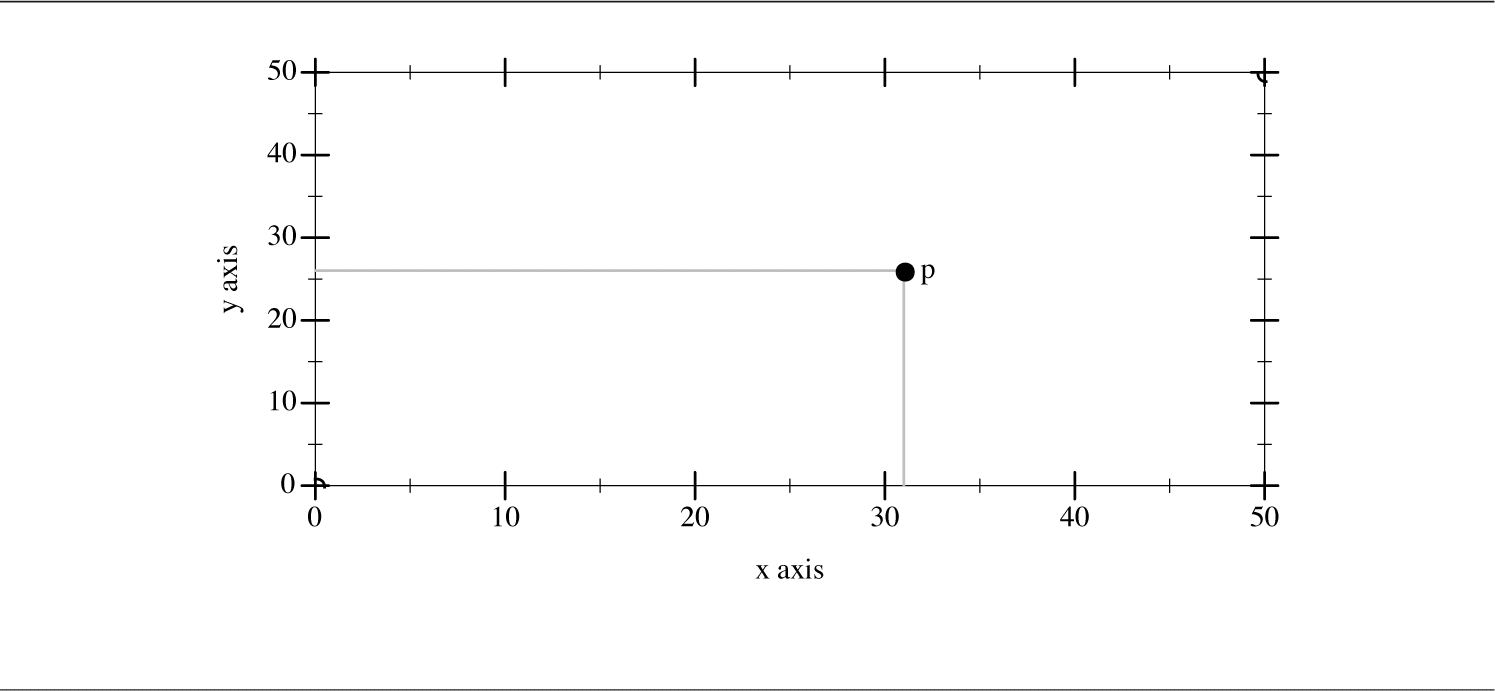
\includegraphics[width=0.45\textwidth]{images/00095.png}
  \caption{笛卡尔坐标系中的二维点 $(x, y)$}
  \label{fig:cartesian_point}
\end{figure}

为了表示这样的点，BSL 提供了一种内置的数据构造机制——\code{posn}。我们可以使用构造函数 \code{make-posn} 来创建一个位置结构体：

\begin{lstlisting}[language=BSL]
(make-posn 3 4)
(make-posn 8 6)
(make-posn 5 12)
\end{lstlisting}

在概念上，你可以把结构体想象为一个带有标签与分隔隔板的“盒子”（box）。图~\ref{fig:posn_box} 展示了 \code{(make-posn 3 4)} 在内存中的盒子模型：

\begin{figure}[htbp]
  \centering
  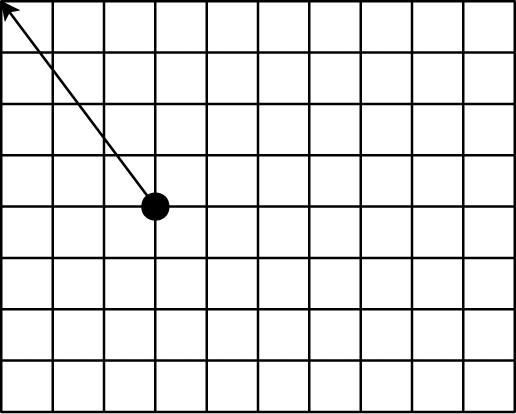
\includegraphics[width=0.35\textwidth]{images/00096.png}
  \caption{posn 结构体的盒子示意模型}
  \label{fig:posn_box}
\end{figure}

这个盒子带有标签 \code{posn}，内部包含两个插槽（slots），分别存放了横坐标 3 与纵坐标 4。

既然能将两个数装入盒子，我们就必然需要手段从盒子中取出它们。BSL 提供了两个\term{选择器}（selectors）：
\begin{itemize}
  \item \code{posn-x}：提取结构体中的 $x$ 字段；
  \item \code{posn-y}：提取结构体中的 $y$ 字段。
\end{itemize}

在 DrRacket 交互区中尝试：

\begin{replbox}
> (define p (make-posn 31 10))
> (posn-x p)
31
> (posn-y p)
10
> (posn-x (make-posn 3 4))
3
> (posn-y (make-posn 3 4))
4
\end{replbox}

选择器 \code{posn-x} 与 \code{posn-y} 就像精密的镊子，可以穿透盒子的外壳，将指定字段的数据直接提取出来。

% ==============================================================================
\section{posn 的求值与计算}
\label{sec:5.2_computing_with_posns}
% ==============================================================================

理解结构体的关键在于理解其在算术求值中的等价替换规则。针对 \code{posn}，BSL 增加了两条极其简单的归约公理：

\begin{notebox}[posn 选择器的求值规则]
对于任意两个值 $v_1$ 和 $v_2$：
\begin{align*}
\code{(posn-x (make-posn $v\_1$ $v\_2$))} &\Longrightarrow v_1 \\
\code{(posn-y (make-posn $v\_1$ $v\_2$))} &\Longrightarrow v_2
\end{align*}
也就是说，当一个选择器应用在一个显式的 \code{make-posn} 实例上时，整个表达式在一步计算内直接化简为对应槽位中的值。
\end{notebox}

例如，考虑下面表达式的求值演进：
\begin{lstlisting}[language=BSL]
  (+ (posn-x (make-posn 3 4)) (posn-y (make-posn 3 4)))
== (+ 3 (posn-y (make-posn 3 4)))
== (+ 3 4)
== 7
\end{lstlisting}

\begin{exercise}{结构体表达式手工推演}{63}
单步推演以下表达式的计算过程，写出每一步的替换结果：
\begin{lstlisting}[language=BSL]
(distance-to-0 (make-posn 3 4))
(distance-to-0 (make-posn (* 2 3) (* 2 4)))
(distance-to-0 (make-posn 12 (- 6 1)))
\end{lstlisting}
其中 \code{distance-to-0} 是计算点到原点欧几里得距离的函数：
\begin{lstlisting}[language=BSL]
(define (distance-to-0 ap)
  (sqrt (+ (sqr (posn-x ap)) (sqr (posn-y ap)))))
\end{lstlisting}
\end{exercise}

\begin{exercise}{曼哈顿距离}{64}
在曼哈顿这样的街区中，两点之间的距离不能沿对角线直飞，而必须沿着由正交街道构成的方格网格行走。一个点 $(x, y)$ 到原点 $(0, 0)$ 的\term{曼哈顿距离}（Manhattan distance）定义为：
\[
\text{ManhattanDistance}(p) = |x| + |y|
\]
设计函数 \code{manhattan-distance}，接收一个 \code{Posn} 作为输入，计算并返回其到原点的曼哈顿距离。
\end{exercise}

% ==============================================================================
\section{使用 posn 进行编程}
\label{sec:5.3_programming_with_posn}
% ==============================================================================

在程序设计配方的语境下，\code{Posn} 是一个全新的数据集合。我们要编写处理 \code{Posn} 的函数，首先必须明确其数据定义与解释：

\begin{lstlisting}[language=BSL]
; 一个 Posn 是一个结构体：
;   (make-posn Number Number)
; 解释：表示二维笛卡尔坐标系中的一个点，包含 x 坐标与 y 坐标
\end{lstlisting}

图~\ref{fig:distance_to_0_design} 展示了设计 \code{distance-to-0} 函数的完整历程：从签名、目的说明、功能测试，到针对结构体的模板，再到最终的函数体。

\begin{figure}[htbp]
  \centering
  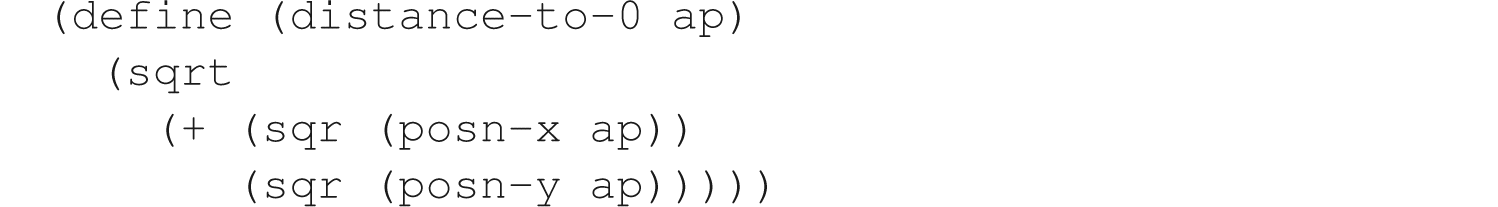
\includegraphics[width=0.85\textwidth]{images/00098.png}
  \caption{distance-to-0 函数的设计全貌与测试}
  \label{fig:distance_to_0_design}
\end{figure}

注意在编写模板时，由于输入参数 \code{ap} 是一个 \code{posn}，模板会立即写出提取其各字段的表达式：
\begin{lstlisting}[language=BSL]
(define (distance-to-0 ap)
  (... (posn-x ap) ... (posn-y ap) ...))
\end{lstlisting}
这种从数据定义直接推导模板的能力，正是设计配方的核心威力所在。

% ==============================================================================
\section{定义结构体类型}
\label{sec:5.4_defining_structure_types}
% ==============================================================================

虽然 \code{posn} 非常方便，但它只有两个字段，且语义固定为“二维坐标”。现实中的问题需要各种各样不同的复合数据：电影信息、三维向量、学生档案、颜色RGB值等。为此，BSL 赋予了程序员定义全新结构体类型的权力——\code{define-struct}。

\code{define-struct} 的通用语法形式为：

\begin{lstlisting}[language=BSL]
(define-struct StructureName [FieldName_1 ... FieldName_N])
\end{lstlisting}

例如：
\begin{lstlisting}[language=BSL]
(define-struct entry [name phone email])
\end{lstlisting}

这个单行定义施展了令人惊叹的魔法：它不是定义了一个变量，而是瞬间向 BSL 的语言环境中注入了一整套全新的函数！
对于一个拥有 $N$ 个字段的结构体类型定义：
\begin{enumerate}
  \item 一个\term{构造函数}（constructor）：名字为 \code{make-StructureName}，接收 $N$ 个参数，返回该结构体的一个新实例；
  \item $N$ 个\term{选择器}（selectors）：名字形如 \code{StructureName-FieldName\_i}，用于提取第 $i$ 个字段的值；
  \item 一个\term{类型谓词}（predicate）：名字为 \code{StructureName?}，接收任意值，判断该值是否属于此结构体类型。
\end{enumerate}

\begin{figure}[htbp]
  \centering
  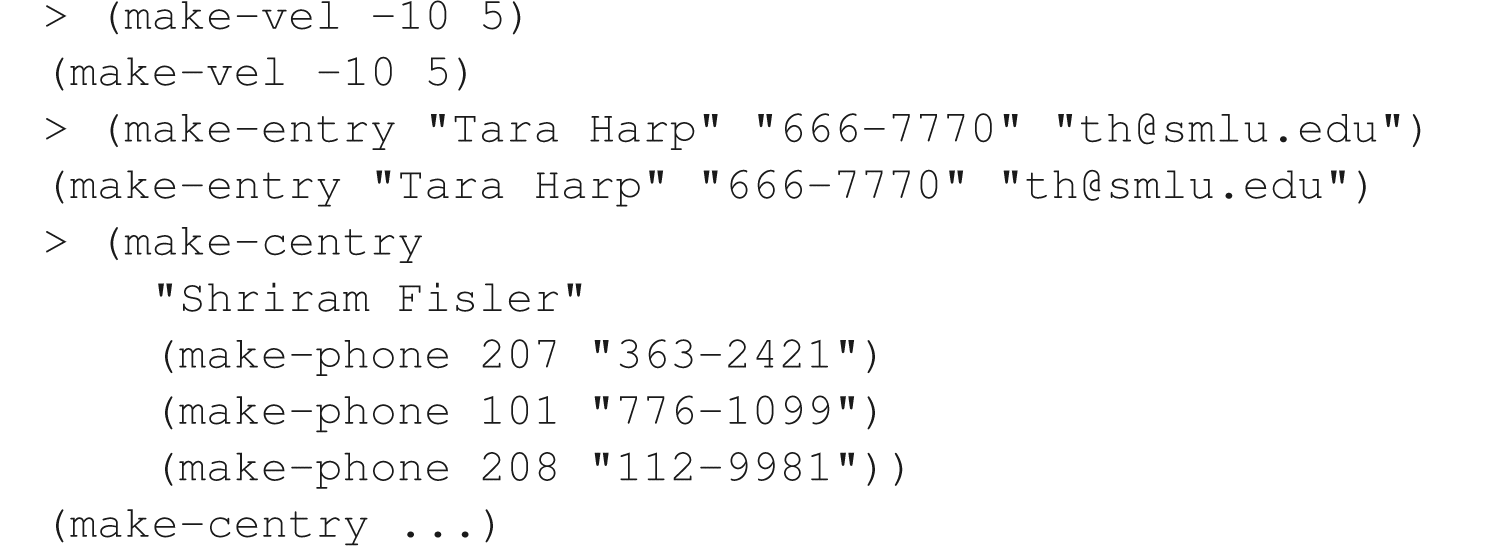
\includegraphics[width=0.75\textwidth]{images/00103.png}
  \caption{define-struct 自动派生的一组函数簇}
  \label{fig:struct_functions_derived}
\end{figure}

例如，执行 \code{(define-struct entry [name phone email])} 之后，你立刻获得了：
\begin{itemize}
  \item 构造函数：\code{make-entry}
  \item 选择器：\code{entry-name}, \code{entry-phone}, \code{entry-email}
  \item 谓词：\code{entry?}
\end{itemize}

\begin{exercise}{分析结构体类型定义}{65}
仔细研读以下结构体类型定义：
\begin{lstlisting}[language=BSL]
(define-struct movie [title director year])
(define-struct person [name hair eyes phone])
(define-struct pet [name number])
(define-struct CD [artist title price])
(define-struct sweater [material size producer])
\end{lstlisting}
分别写出每一个定义所派生出的构造函数、选择器以及类型谓词的名字和参数个数。
\end{exercise}

\begin{exercise}{创建结构体实例}{66}
回顾练习~\ref{ex:65} 中的结构体定义。对每个字段应当存放何种类型的值作出合理的推断与设计，然后为每个结构体类型至少创建一个实际的具体实例。
\end{exercise}

\begin{exercise}{弹跳球的嵌套数据表示}{67}
考虑在画布上弹跳的小球。一个小球不仅有位置，还有移动速度。这里给出一种嵌套结构表示：
\begin{lstlisting}[language=BSL]
(define-struct balld [location velocity])
(define-struct vel [deltax deltay])
\end{lstlisting}
请写出创建一个位于 $(10, 20)$、以水平速度 5 垂直速度 $-3$ 移动的小球的实例创建表达式。
\end{exercise}

\begin{exercise}{扁平化的弹跳球表示}{68}
作为对比，另一种表示法直接使用拥有四个字段的扁平结构体：
\begin{lstlisting}[language=BSL]
(define-struct ballf [x y deltax deltay])
\end{lstlisting}
创建与练习~\ref{ex:67} 相同物理含义的小球实例，并比较两种数据组织的优缺点。
\end{exercise}

% ==============================================================================
\section{使用结构体计算}
\label{sec:5.5_computing_with_structures}
% ==============================================================================

结构体实例的盒子模型同样适用于用户自定义结构体。图~\ref{fig:entry_box} 展示了 \code{entry} 结构体的内存示意图：

\begin{figure}[htbp]
  \centering
  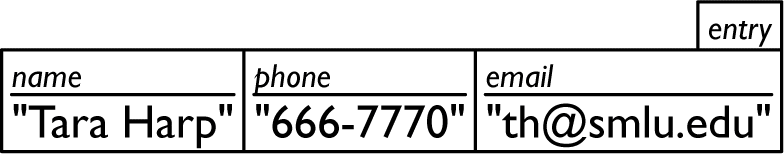
\includegraphics[width=0.65\textwidth]{images/00101.png}
  \caption{entry 结构体实例的盒子模型}
  \label{fig:entry_box}
\end{figure}

针对用户自定义结构体，BSL 的核心计算法则直接推广为：

\begin{notebox}[结构体选择器的代数公理]
设某结构体类型定义为 \code{(define-struct StructureName [f\_1 ... f\_N])}。
对于任意 $N$ 个值 $v_1, \dots, v_N$：
\[
\code{(StructureName-}f_i\code{ (make-StructureName } v_1 \code{ } \dots \code{ } v_N \code{))} \Longrightarrow v_i \quad (1 \le i \le N)
\]
此外，类型谓词满足：
\begin{align*}
\code{(StructureName? (make-StructureName } v_1 \code{ } \dots \code{ } v_N \code{))} &\Longrightarrow \code{\#true} \\
\code{(StructureName? } \text{other-value} \code{)} &\Longrightarrow \code{\#false}
\end{align*}
\end{notebox}

\begin{exercise}{绘制盒子图}{69}
为你在练习~\ref{ex:66} 中创建的所有结构体实例绘制类似图~\ref{fig:entry_box} 的盒子示意图。
\end{exercise}

\begin{exercise}{写出代数公理}{70}
为以下两个结构体类型分别完整列出其选择器和谓词的代数计算公理：
\begin{lstlisting}[language=BSL]
(define-struct centry [name home office cell])
(define-struct phone [area number])
\end{lstlisting}
\end{exercise}

\begin{exercise}{结构体字段访问求值验证}{71}
在 DrRacket 定义区输入以下定义，然后预测并在交互区验证输出结果：
\begin{lstlisting}[language=BSL]
(define-struct posn [x y]) ; 注意：BSL 内置了 posn，无需重复定义
(define p1 (make-posn 2 3))
(define p2 (make-posn (posn-y p1) (posn-x p1)))
\end{lstlisting}
预测 \code{(posn-x p2)} 与 \code{(posn-y p2)} 的计算结果。
\end{exercise}

% ==============================================================================
\section{结构体编程}
\label{sec:5.6_programming_with_structures}
% ==============================================================================

在实际业务中，我们经常需要对结构体进行“更新”（update）。请牢记：\textbf{在函数式编程中，数据是不可变的（immutable）}。所谓“更新”一个点，绝不是去修改原有点的字段，而是根据旧点的值计算出一个\textbf{全新的结构体实例}！

例如，设计一个函数 \code{posn-up-x}，它接收一个点 \code{p} 和一个新坐标 \code{n}，返回一个横坐标为 \code{n}、纵坐标保持与 \code{p} 相同的新点：

\begin{lstlisting}[language=BSL]
; Posn Number -> Posn
; 生成一个新的 Posn，其 x 坐标为 n，y 坐标取自 p
(check-expect (posn-up-x (make-posn 3 4) 10) (make-posn 10 4))

(define (posn-up-x p n)
  (make-posn n (posn-y p)))
\end{lstlisting}

\begin{exercise}{电话结构体数据定义}{72}
为如下三字段电话号码设计数据定义与解释：
\begin{lstlisting}[language=BSL]
(define-struct phone\# [area switch num])
\end{lstlisting}
并给出三个具体的电话号码数据实例。
\end{exercise}

\begin{exercise}{点更新函数 posn-up-x}{73}
完整实现并测试 \code{posn-up-x} 函数，确保其通过所有单元测试。
\end{exercise}

\begin{exercise}{红点点击世界程序}{74}
编写一个世界程序，其世界状态为一个 \code{Posn}。画布初始时在 $(0, 0)$ 处绘制一个半径为 3 的红点；当用户在画布上点击鼠标时，红点立即跃迁到鼠标点击的坐标位置。
\end{exercise}

\begin{exercise}{UFO 移动函数}{75}
设计函数 \code{ufo-move}，接收一个表示当前位置的 \code{Posn} 和表示速度的 \code{Vel} 结构体，返回下一时刻小球的新位置 \code{Posn}。
\end{exercise}

% ==============================================================================
\section{数据的全集与领域}
\label{sec:5.7_the_universe_of_data}
% ==============================================================================

当我们引入结构体之后，程序中所处理的数据世界发生了根本性的飞跃。

在图~\ref{fig:universe_simple} 中，原始数据宇宙只包含离散的基本类型原子（数、字符串、图像、布尔值）。

\begin{figure}[htbp]
  \centering
  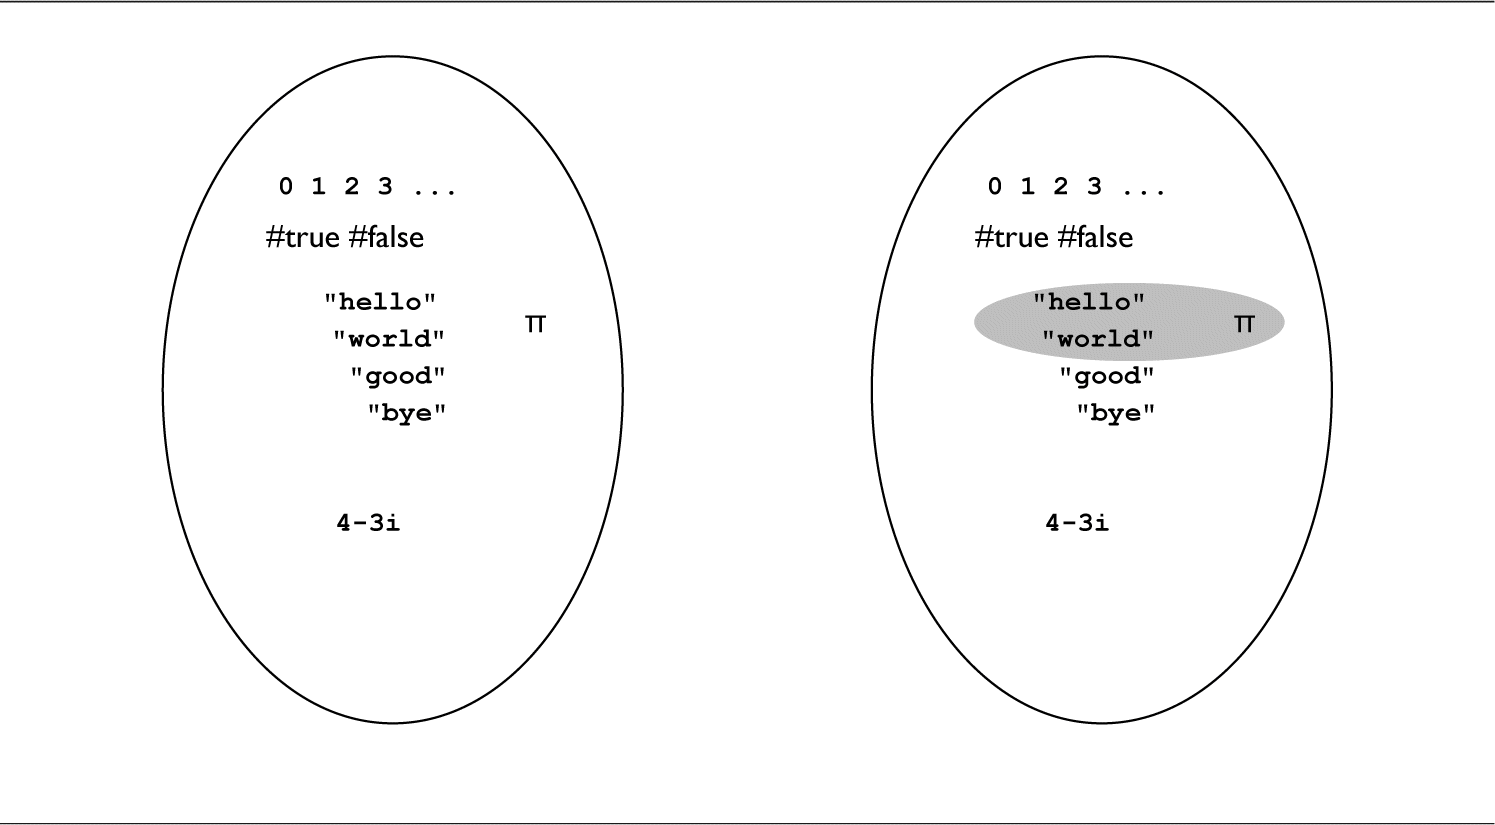
\includegraphics[width=0.65\textwidth]{images/00107.png}
  \caption{原始的基本数据全集}
  \label{fig:universe_simple}
\end{figure}

而每当我们在程序中书写一行 \code{(define-struct S [f\_1 ... f\_N])}，数据宇宙中就立即诞生了一个全新的、无限庞大的星系（见图~\ref{fig:universe_with_structs}）——所有由 \code{make-S} 生成的实例构成了一个全新的数据子集！

\begin{figure}[htbp]
  \centering
  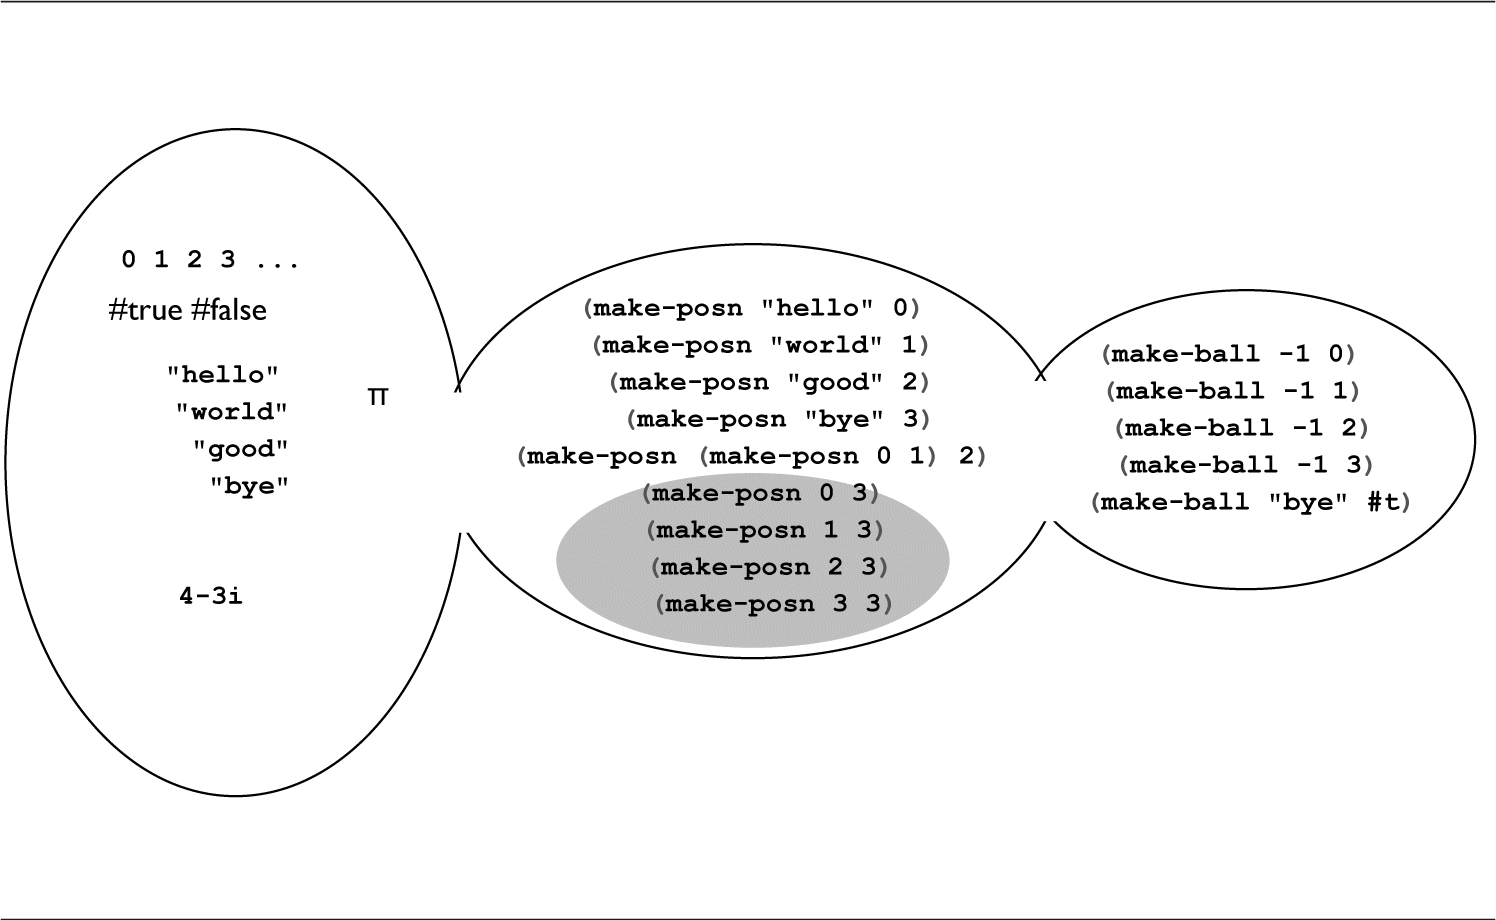
\includegraphics[width=0.7\textwidth]{images/00108.png}
  \caption{引入结构体后无限膨胀的数据宇宙}
  \label{fig:universe_with_structs}
\end{figure}

更令人惊叹的是：由于结构体的字段本身又可以存放任意数据值（包括另一个结构体实例！），我们获得了无限层级嵌套与组合复杂世界现实的能力。

\begin{exercise}{为结构体写出严密的数据定义}{76}
回顾练习~\ref{ex:65} 中的结构体定义（movie, person, pet, CD, sweater）。为每一个结构体类型写出规范的、包含各字段类型约束与物理现实解释的数据定义。
\end{exercise}

\begin{exercise}{时间结构体}{77}
提供一个结构体类型定义与数据定义，用于精确表示自午夜（00:00:00）以来经过的时间（包含小时、分钟和秒）。
\end{exercise}

\begin{exercise}{三字母单词结构体}{78}
定义一个表示由三个字母组成的单词的结构体类型定义及数据定义。
\end{exercise}

\begin{exercise}{复杂场景数据表示}{79}
为以下实体分别设计结构体与数据定义：
\begin{enumerate}
  \item 屏幕上彩色的几何图形；
  \item 包含姓名、年龄、住址的个人档案；
  \item 包含品种、晶片编号、疫苗注射状态的宠物犬；
  \item 具有弹药量、伤害值和耐久度的武器。
\end{enumerate}
\end{exercise}

% ==============================================================================
\section{针对结构体的设计配方}
\label{sec:5.8_designing_with_structures}
% ==============================================================================

当函数的输入参数包含结构体时，程序设计配方展现出极其清晰的形式化指引：

\begin{recipebox}{设计处理结构体的函数}
\begin{enumerate}
  \item \textbf{数据定义}：
    \begin{itemize}
      \item 使用 \code{(define-struct TypeName [f\_1 ... f\_N])} 定义结构体形态；
      \item 编写对应的数据定义注释，明确指定每个字段的类型取值范围；
      \item 给出每个字段在现实世界中的业务解释（Interpretation）。
    \end{itemize}
  \item \textbf{签名、目的说明与函数头}：在签名中以自定义结构体名称（首字母大写，如 \code{Posn}, \code{Entry}）作为输入或输出类型。
  \item \textbf{功能示例}：在创建示例时，必须使用构造函数 \code{make-TypeName} 实例化具体的数据对象。
  \item \textbf{函数模板}：\textbf{对于结构体参数，无条件提取所有选择器！}
\begin{lstlisting}[language=BSL]
(define (fn-for-struct s)
  (... (TypeName-f_1 s) ...
   ... (TypeName-f_2 s) ...
   ...
   ... (TypeName-f_N s) ...))
\end{lstlisting}
    模板忠实反映了“盒子”里的每一个插槽。你在写函数体之前，就已经清楚拥有了哪些现成的零件。
  \item \textbf{函数体实现}：利用提取出的各字段数据，组合出最终的运算结果。若输出也是结构体，则调用相应的构造函数生成新实例。
  \item \textbf{自动化测试}：使用 \code{check-expect} 校验所有测试用例。
\end{enumerate}
\end{recipebox}

\begin{exercise}{写出结构体模板}{80}
为练习~\ref{ex:65} 中的五个结构体类型分别写出其标准处理函数的函数模板。
\end{exercise}

\begin{exercise}{时间转秒数}{81}
设计函数 \code{time->seconds}，接收一个练习~\ref{ex:77} 中定义的时间结构体，计算并返回自午夜以来累计流逝的总秒数。
\end{exercise}

\begin{exercise}{三字母单词匹配}{82}
设计函数 \code{compare-word}，接收两个练习~\ref{ex:78} 中定义的三字母单词结构体，逐个字母比对并返回一个指示每个位置是否匹配的新单词结构体。
\end{exercise}

% ==============================================================================
\section{世界程序中的结构体}
\label{sec:5.9_structure_in_the_world}
% ==============================================================================

在第 3 章中，世界程序的 WorldState 只能是一个单一标量（数或字符串）。现在有了结构体，世界状态可以同时追踪任意多个运动物体或环境参数！

例如，如果一个太空射击游戏同时包含飞船坐标、外星人飞碟坐标以及发射出的导弹坐标，我们只需定义：
\begin{lstlisting}[language=BSL]
(define-struct space-game [ship ufo missile])
\end{lstlisting}
世界状态在每一帧时钟滴答中被整体更新，渲染函数则从各个字段中分别提取坐标进行分层绘制。

% ==============================================================================
\section{图形文本编辑器}
\label{sec:5.10_a_graphical_editor}
% ==============================================================================

作为结构体威力的绝佳展示，我们来设计一个单行交互式图形文本编辑器（Graphical Text Editor）！

编辑器展现为一个输入框，包含一段文字和一个垂直光标。用户在键盘上输入字母时，字符插入到光标所在位置；按退格键（\code{"\textbackslash b"}）时删除光标左侧的字符；按左方向键（\code{"left"}）或右方向键（\code{"right"}）时光标左右移动。

如何用数据表示这个编辑器呢？
直觉上，你可能会想用一个长字符串加一个光标索引数字（Index）。但处理字符串切片和索引加减极易出现“差一错误”（off-by-one error）。
HtDP 传授了一个精妙绝伦的数据表示——\textbf{将文本按光标拆分为两段字符串}（见图~\ref{fig:editor_split}）：
\begin{itemize}
  \item \code{pre}：光标左侧的所有文本；
  \item \code{post}：光标右侧的所有文本。
\end{itemize}

\begin{figure}[htbp]
  \centering
  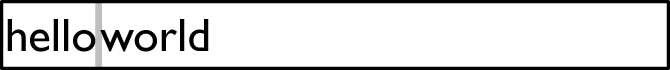
\includegraphics[width=0.7\textwidth]{images/00110.png}
  \caption{光标切分文本模型示意图}
  \label{fig:editor_split}
\end{figure}

\begin{lstlisting}[language=BSL]
(define-struct editor [pre post])
; 一个 Editor 是一个结构体：
;   (make-editor String String)
; 解释：(make-editor s t) 表示光标位于字符串 s 和 t 之间
\end{lstlisting}

例如：\code{(make-editor "hello " "world")} 表示文本为 \code{"hello world"}，光标位于空格与 \code{"w"} 之间。

\begin{figure}[htbp]
  \centering
  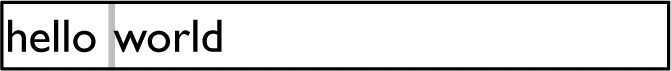
\includegraphics[width=0.45\textwidth]{images/00111.png}
  \caption{editor 结构体实例的盒子模型}
  \label{fig:editor_box}
\end{figure}

\begin{figure}[htbp]
  \centering
  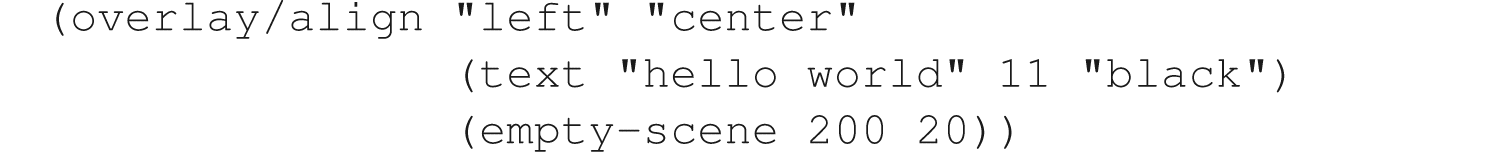
\includegraphics[width=0.85\textwidth]{images/00112.png}
  \caption{文本编辑器的渲染函数 render}
  \label{fig:editor_render}
\end{figure}

\begin{exercise}{编辑器渲染函数}{83}
设计函数 \code{render}，接收一个 \code{Editor}，生成包含文本与垂直红色光标线段的图像（如图~\ref{fig:editor_render} 所示）。
\end{exercise}

\begin{exercise}{按键编辑逻辑 edit}{84}
设计函数 \code{edit}，接收一个 \code{Editor} 和一个 \code{KeyEvent}，返回更新后的 \code{Editor}。必须严谨处理以下情况：
\begin{itemize}
  \item 普通单字符按键（长度为 1 的非控制字符串）：追加到 \code{pre} 的末尾；
  \item \code{"\textbackslash b"}（退格）：删除 \code{pre} 的最后一个字符；若 \code{pre} 为空则忽略；
  \item \code{"left"}（左移光标）：将 \code{pre} 的最后一个字符转移到 \code{post} 的开头；
  \item \code{"right"}（右移光标）：将 \code{post} 的首字符转移到 \code{pre} 的末尾；
  \item \code{"\textbackslash t"} 或 \code{"\textbackslash r"} 等控制字符：直接忽略，保持原样。
\end{itemize}
\end{exercise}

\begin{exercise}{组装运行图形编辑器}{85}
编写 \code{run} 函数，接收一个初始文本字符串，调用 \code{big-bang} 启动交互式文本编辑器！
\end{exercise}

\begin{exercise}{防止文本超出边界}{86}
如果用户持续输入，文本可能会超出画布边界。修改 \code{edit} 函数，若新字符会导致文本宽度超出画布，则拒绝输入。
\end{exercise}

\begin{exercise}{基于字符串与索引的替代实现}{87}
尝试使用第一种思路（一个完整字符串加一个整数光标索引）重做上述编辑器练习，对比两套方案的实现复杂度与代码优雅性。
\end{exercise}

% ==============================================================================
\section{更多虚拟宠物}
\label{sec:5.11_more_virtual_pets}
% ==============================================================================

在第 3.7 节中，我们分别独立编写了行走的小猫世界程序与心情计世界程序。现在借助结构体，我们可以将它们合二为一，打造一个真正鲜活的虚拟宠物！

\begin{figure}[htbp]
  \centering
  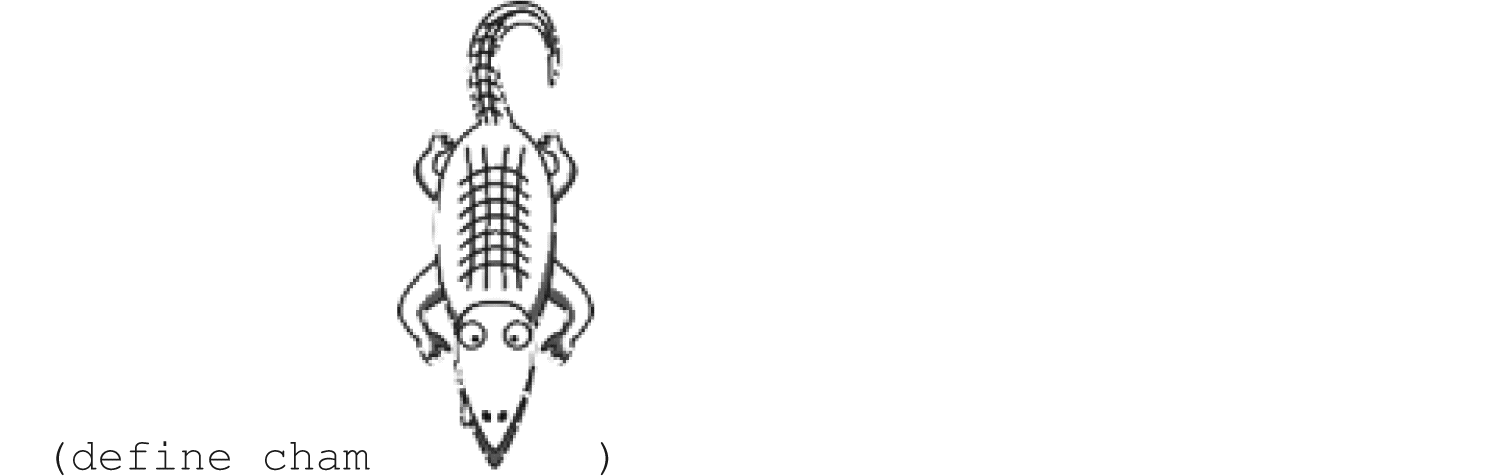
\includegraphics[width=0.6\textwidth]{images/00113.png}\\[1ex]
  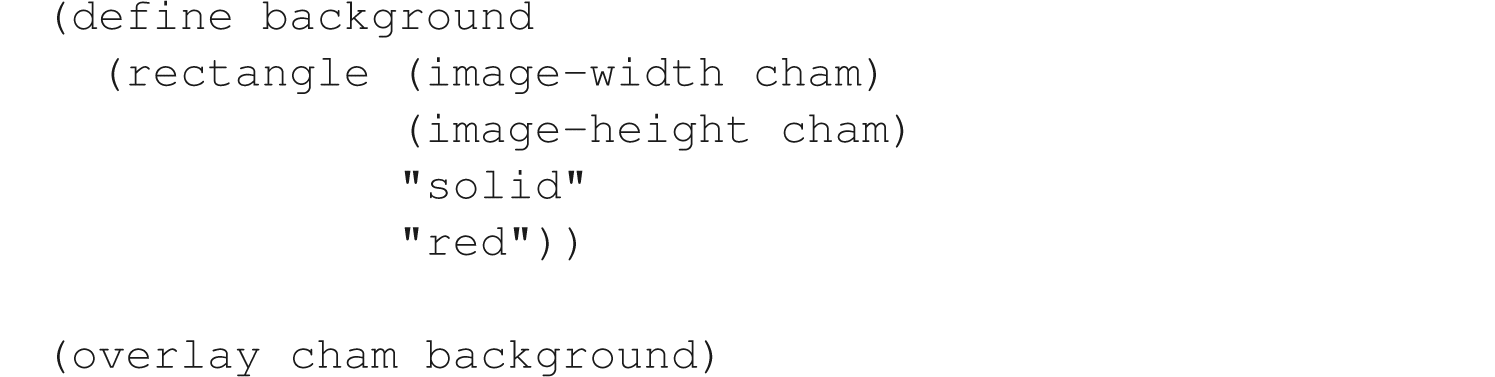
\includegraphics[width=0.6\textwidth]{images/00114.png}
  \caption{行走的小猫（上）与快乐指数仪表盘（下）}
  \label{fig:cat_and_gauge}
\end{figure}

\begin{exercise}{虚拟小猫的数据定义 VCat}{88}
定义一个结构体类型与数据定义 \code{VCat}，同时记录小猫的水平坐标 $x$ 与当前的快乐值 $h$。
\end{exercise}

\begin{exercise}{打造 happy-cat 世界程序}{89}
设计 \code{happy-cat} 程序，在画布上方显示小猫，下方显示心情指数进度条。小猫每前进一步，心情便略微下滑；用户可以通过喂食（下方向键）或抚摸（上方向键）来提升小猫的快乐值。
\end{exercise}

\begin{exercise}{停止条件：猫咪伤心过度}{90}
利用 \code{stop-when} 子句，当小猫的快乐值跌落至 0 时立即终止程序。
\end{exercise}

\begin{exercise}{双向行走的猫咪}{91}
扩展 \code{VCat} 结构体以记录移动方向。当小猫触碰画布边缘时，自动掉头向反方向行走。
\end{exercise}

\begin{figure}[htbp]
  \centering
  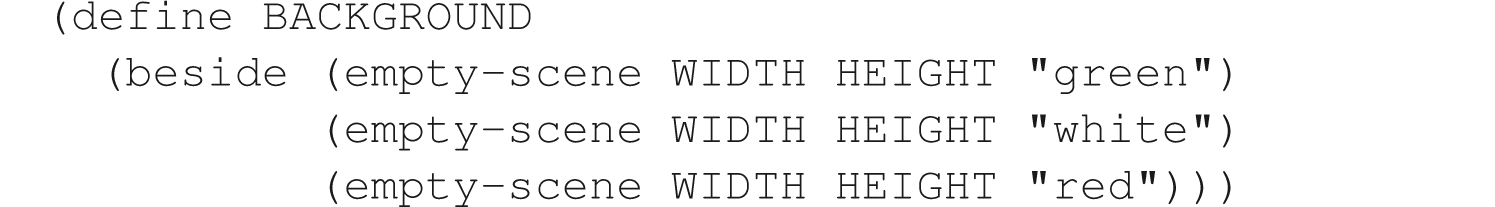
\includegraphics[width=0.7\textwidth]{images/00115.png}
  \caption{三色背景上行走的变色龙}
  \label{fig:cham_tricolor}
\end{figure}

\begin{exercise}{变色龙虚拟宠物}{92}
设计 \code{cham} 虚拟变色龙程序。变色龙从左至右在画布上漫步，同样拥有饥饿与快乐机制。
\end{exercise}

\begin{exercise}{三色背景上的变色龙}{93}
复制并修改练习~\ref{ex:92} 的程序，使得变色龙行走在一个由红、白、绿三色竖条纹构成的背景上，并且身体颜色会随着按键改变。
\end{exercise}
